\section{EverMemOS}

\subsection{Framework Overview}

Drawing inspiration from the biological engram lifecycle \cite{josselyn2015finding}, EverMemOS follows a three-phase workflow (Figure~\ref{fig:workflow}): (1) \textbf{Episodic Trace Formation} encodes interaction streams into \textit{MemCells}; (2) \textbf{Semantic Consolidation} organizes MemCells into \textit{MemScenes} and updates user profiles; and (3) \textbf{Reconstructive Recollection} performs \textit{MemScene}-guided retrieval under the principle of necessity and sufficiency.

\begin{figure*}[t]
    \centering
    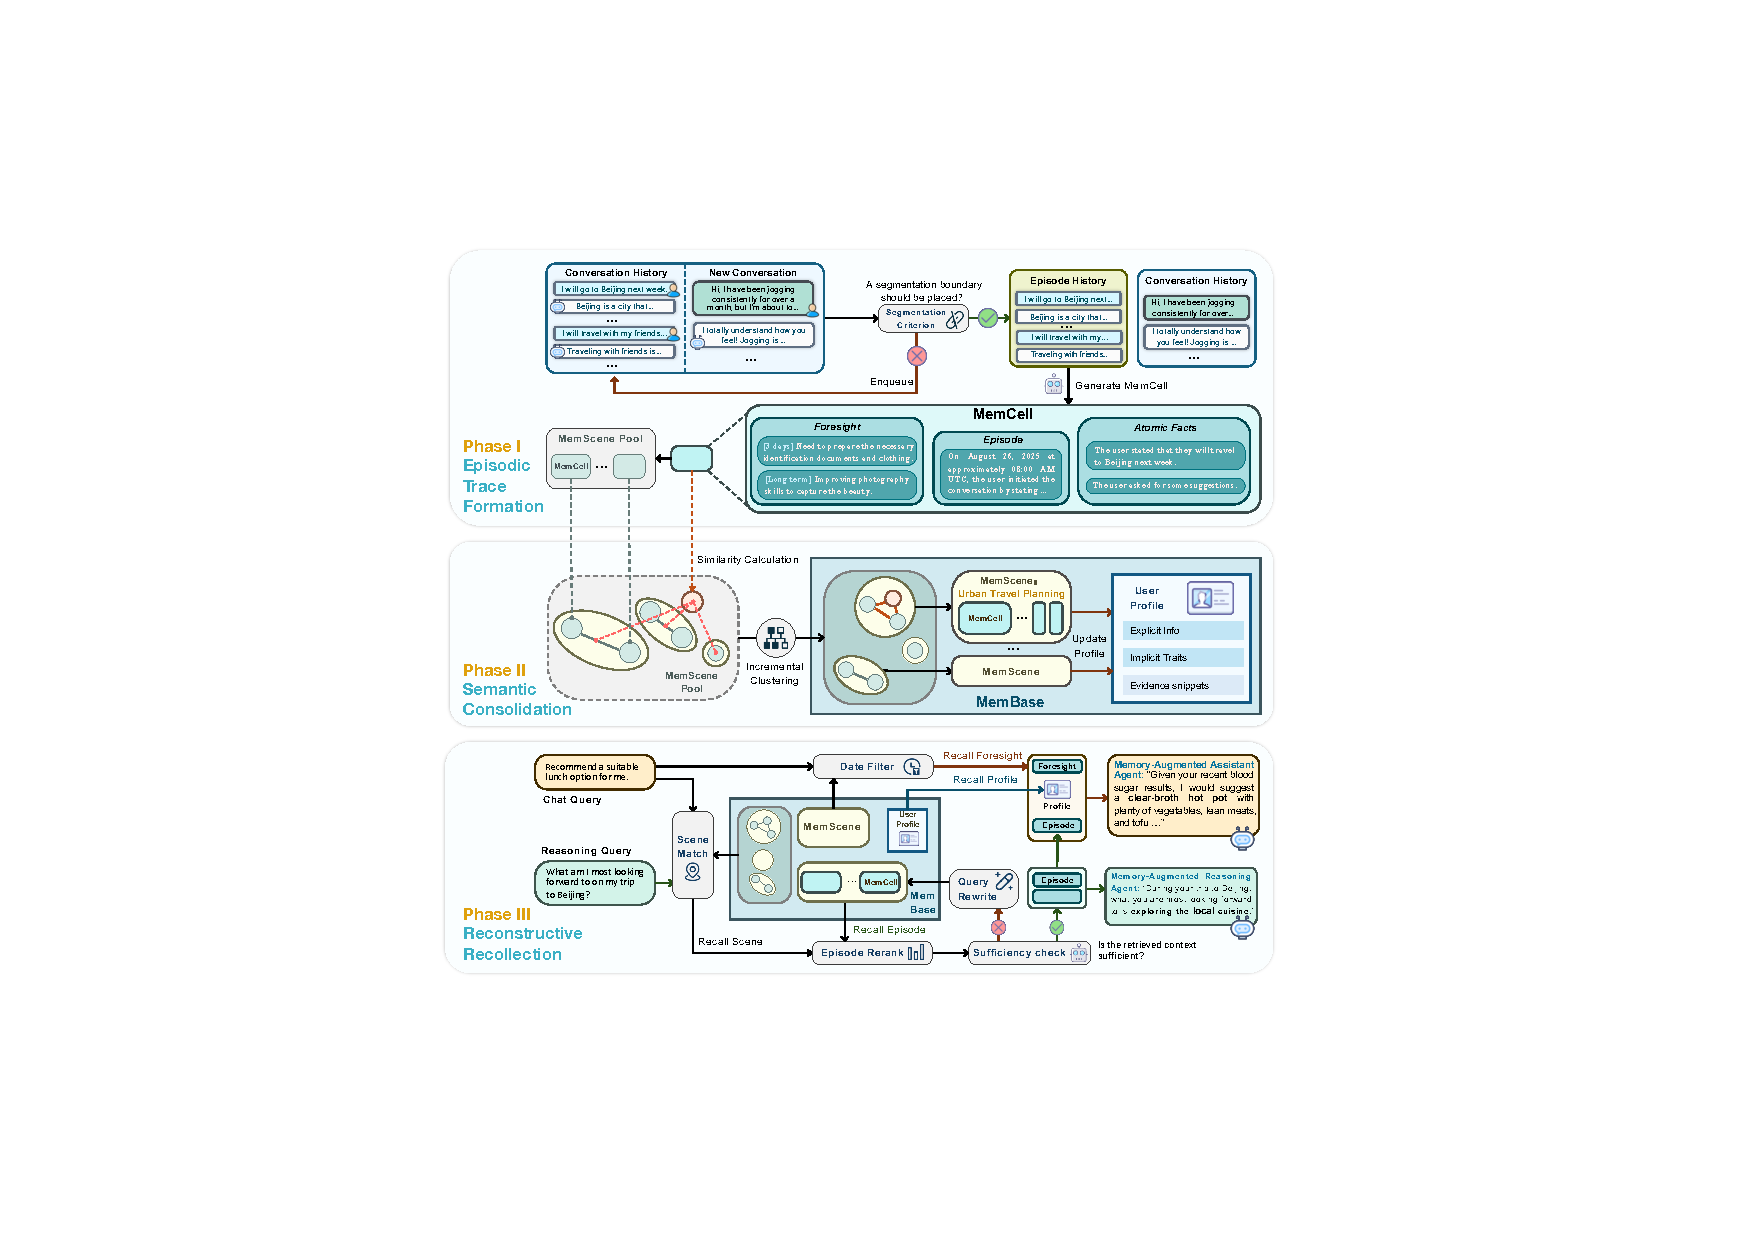
\includegraphics[width=0.93\textwidth]{figure/main.pdf}
    \vspace{-2mm}
    \caption{The EverMemOS workflow mirrors an engram-inspired memory lifecycle: (1) \textbf{Episodic Trace Formation} segments continuous dialogue into \textit{MemCells} with episodes, atomic facts, and time-bounded foresight. (2) \textbf{Semantic Consolidation} organizes MemCells into \textit{MemScenes} and updates a user profile. (3) \textbf{Reconstructive Recollection} performs \textit{MemScene}-guided retrieval to compose the necessary and sufficient context.}
    \vspace{-4mm}
    \label{fig:workflow}
\end{figure*}

\subsection{Memory Primitives}
\label{sec:primitives}

At the core of EverMemOS is the \textbf{MemCell}, the atomic unit bridging low-level data and high-level semantics. Formally, a MemCell $c$ is a tuple $c = (E, \mathcal{F}, P, M)$, where:
\begin{itemize}
    \item $E$ (\textbf{Episode}): A concise third-person narrative of the event, serving as the semantic anchor.
    \item $\mathcal{F} = \{f_1, \dots, f_n\}$ (\textbf{Atomic Facts}): Discrete, verifiable statements derived from $E$ for high-precision matching.
    \item $P$ (\textbf{Foresight}): Forward-looking inferences (prospections; e.g., plans and temporary states) annotated with validity intervals $[t_{start}, t_{end}]$ to support temporal awareness.
    \item $M$ (\textbf{Metadata}): Contextual grounding including timestamps and source pointers.
\end{itemize}
This structure turns memory from a static record ($E, \mathcal{F}$) into a temporally grounded representation that also supports \textbf{Foresight} ($P$).

\subsection{Phase I: Episodic Trace Formation}
Grounded in the engram concept \cite{josselyn2015finding}, this first phase transforms the unbounded stream of interaction history $\mathcal{D}=\{d_1,\ldots,d_T\}$ into discrete, stable memory traces (MemCells). This process adopts a three-step pipeline to distill semantic signal from noisy interaction data:

\paragraph{Contextual Segmentation} To discretize continuous streams, a \textbf{Semantic Boundary Detector} processes interactions via a sliding window. Upon detecting a topic shift, accumulated turns are encapsulated as a raw \textit{episode history}. We implement this step via LLM prompting; while boundary detection is not perfect, we find it robust in downstream evaluation (see Table~\ref{tab:locomo-bound}).

\paragraph{Narrative Synthesis} To resolve dialogue redundancy and ambiguity, the episode history is synthesized into a high-fidelity \textbf{Episode} ($E$). This rewriting process produces a concise, third-person narrative with resolved coreferences, establishing a stable semantic anchor.

\paragraph{Structural Derivation} From $E$, the system extracts \textbf{Atomic Facts} ($\mathcal{F}$) for precise matching and generates \textbf{Foresight} signals ($P$) with inferred validity intervals (e.g., distinguishing temporary "flu" from permanent "graduation"). Concretely, we prompt the LLM over the rewritten Episode $E$ to output a constrained schema of Atomic Facts and Foresight signals with validity intervals $[t_{start}, t_{end}]$. These components are bundled with metadata $M$ to form the final MemCell $c$.


\subsection{Phase II: Semantic Consolidation}
Inspired by systems consolidation \cite{mcgaugh2000memory}, EverMemOS employs an online mechanism that organizes MemCells into higher-order structures to transition from transient episodes to stable long-term knowledge.

\paragraph{Incremental Semantic Clustering}
EverMemOS organizes memory dynamically. When a new MemCell $c$ arrives, the system computes its embedding and retrieves the nearest \textbf{MemScene} centroid. If similarity exceeds a threshold $\tau$, $c$ is assimilated and the scene representation is incrementally updated; otherwise, a new \textbf{MemScene} is instantiated. This online process maintains thematic structure in real-time without batch reprocessing.

\paragraph{Scene-Driven Profile Evolution}
Scene-level consolidation can also update a compact \textbf{User Profile} from aggregated evidence. When a new MemCell is assimilated into a \textbf{MemScene}, EverMemOS updates a concise scene summary and refreshes the user profile by prompting over these summaries (rather than individual turns), helping separate stable traits from temporary states. We maintain a compact profile of \emph{explicit facts} (including time-varying measurements) and \emph{implicit traits}, updated online from scene summaries with recency-aware updates and conflict tracking (Appendix~\ref{sec:profile_example}).

\subsection{Phase III: Reconstructive Recollection}
Building on theories of reconstructive memory \cite{schacter2008searching}, retrieval in EverMemOS is modeled not as a static lookup but as an active \textbf{Reconstruction} process, guided by the principle of \textit{necessity and sufficiency}. Given a query $q$, EverMemOS performs \textbf{agentic retrieval} grounded in \textit{MemScenes}.

\paragraph{MemScene Selection} We first compute relevance between the query and all MemCells by fusing dense and BM25 retrieval over their Atomic Facts $\mathcal{F}$ via Reciprocal Rank Fusion (RRF). We then score each MemScene by the maximum relevance among its constituent MemCells and select a small set of the highest-scoring MemScenes.

\paragraph{Episode and Foresight Filtering} Within the selected MemScenes, we pool Episodes from their constituent MemCells and \textbf{re-rank} them to select a compact set for downstream inference. We then apply \textbf{Foresight Filtering}, retaining only time-valid Foresight whose validity intervals satisfy $t_{now}\in[t_{start}, t_{end}]$ (discarding expired ones).

\paragraph{Agentic Verification and Query Rewriting} The retrieved context is evaluated by an LLM-based verifier for sufficiency. If it is deemed insufficient, the system triggers a \textbf{query rewriting} step to supplement retrieval; otherwise, the context is passed to the downstream module. Prompt templates are provided in Appendix~\ref{sec:agentic_prompts}.

\paragraph{Task Modes} We consider two downstream settings that share the same retrieval pipeline: \textbf{Memory-Augmented Reasoning} and \textbf{Memory-Augmented Chat}. For \textit{Reasoning}, we use the retrieved Episodes as context for benchmark evaluation. For \textit{Chat}, the composed context additionally incorporates the User Profile and time-valid Foresight signals, filtered by the current time $t_{now}\in[t_{start}, t_{end}]$; since these capabilities are not covered by existing reasoning benchmarks, we present them through qualitative case studies.